\documentclass[a4paper,12pt]{article} % This defines the style of your paper
\usepackage[brazilian]{babel} 
\usepackage[top = 2.5cm, bottom = 2.5cm, left = 2.5cm, right = 2.5cm]{geometry} 

\usepackage[T1]{fontenc}
\usepackage[utf8]{inputenc}

\usepackage{multirow} 
\usepackage{booktabs}
\usepackage{amsmath}
\usepackage{graphicx} 
\usepackage{amsmath}
\usepackage{setspace}
\setlength{\parindent}{0in}

% Package to place figures where you want them.
\usepackage{float}

% The fancyhdr package let's us create nice headers.
\usepackage{fancyhdr}

% To make our document nice we want a header and number the pages in the footer.

\pagestyle{fancy} % With this command we can customize the header style.

\fancyhf{} % This makes sure we do not have other information in our header or footer.

\lhead{\footnotesize Atividade sobre LaTex}% \lhead puts text in the top left corner. \footnotesize sets our font to a smaller size.

%\rhead works just like \lhead (you can also use \chead)
\rhead{\footnotesize Daniel Magalhães Nunes} %<---- Fill in your lastnames.

% Similar commands work for the footer (\lfoot, \cfoot and \rfoot).
% We want to put our page number in the center.
\cfoot{\footnotesize \thepage} 
\usepackage[most]{tcolorbox}
\definecolor{block-gray}{gray}{0.95}
\newtcolorbox{blockquote}{colback=block-gray,grow to right by=-1mm,grow to left by=-1mm,boxrule=0pt,boxsep=0pt,breakable}

	
\begin{document}
	%%%%%%%%%%%%%%%%%%%%%%%%%%%%%%%%%%%%%%%%%%%%%%%%
	% Title section of the document
	%%%%%%%%%%%%%%%%%%%%%%%%%%%%%%%%%%%%%%%%%%%%%%%%
	
	% For the title section we want to reproduce the title section of the Problem Set and add your names.
	
	\thispagestyle{empty} % This command disables the header on the first page. 
	
	\begin{tabular}{p{15.5cm}} % This is a simple tabular environment to align your text nicely 
		{\large \bf CK0033 - INTRODUÇÃO A COMPUTAÇÃO} \\
		 Universidade Federal do Ceará \\ 
		 Daniel Magalhães Nunes, 376163 \\
		 Francilene da Silva Sales, 485249 \\ 2020.2 \\
		\hline % \hline produces horizontal lines.
		\\
	\end{tabular} % Our tabular environment ends here.
	
	\vspace*{0.3cm} % Now we want to add some vertical space in between the line and our title.
	
	\begin{center} % Everything within the center environment is centered.
		{\Large \bf Trabalho 4 - LaTex} % <---- Don't forget to put in the right number
		\vspace{2mm}
		
	\end{center}  

	\vspace{0.4cm}
	
	\begin{align*}
			H_0: \mu = \mu_0 \\
			H_1: \mu \pm \mu_0
	\end{align*}

	Se a variância $\sigma^2$ for conhecida, a estatística de teste será a Eq. 8.10:
	
	\begin{equation*}
		Z_0 = \frac{\overline{X} - \mu_0}{\sigma / \sqrt{n}}
	\end{equation*}

	Quando $\sigma^2$ for desconhecida, um procedimento lógico será trocar $\sigma$ na Eq. 9.10 pelo desvio-padrão, S, da amostra. A estatística de teste é agora
	
	\begin{blockquote}
		\begin{equation}
			\tag{8.39}
			T_0 = \frac{\overline{X} - \mu_0}{S / \sqrt{n}}
		\end{equation}  
	\end{blockquote}
	
	Uma questão lógica é qual o efeito de trocar $\sigma$ por $S$ na distribuição da estatística $T_0$? Se $n$ for grande, a resposta a essa questão é "muito pouco" e podemos usar o procedimento de teste baseado na distribuição normal da seção 8.2. Entretanto, n é geralmente pequeno na maioria dos problemas de engenharia e nessa situação uma distribuição diferente tem de ser empregada.
	
	\begin{blockquote}
		\begin{center}
			\textbf{\textit{Definição }} 
		\end{center}
		
		Faça $ X_1 $, $ X_2 $, ... , $ X_n $ ser uma amostra aleatória para uma distribuição normal, com média $\mu$  e variância $\sigma^2$ desconhecida. A grandeza
		
		\begin{equation*}
			T = \frac{\overline{X} - \mu_0}{S / \sqrt{n}}
		\end{equation*}
		
		
		tem uma distribuição $ t $, com $ n-1 $ graus de liberdade.
	\end{blockquote}

	A função densidade da probabilidade $t$ é
	\begin{equation*}
		\tag{8.40}
		f(x) = \frac{\Gamma \left[ \left( k + 1 \right) /2 \right] }{\sqrt{ \pi k  }\Gamma \left( k/2 \right)  } . \frac{1}{\left[ \left( x^2 / k \right) + 1  \right]^{\left( k+1 \right)/2 } } - \infty  < x < \infty 
	\end{equation*}

	sendo $k$ o número de graus de liberdade. A média e a variância da distribuição $t$ são mostradas na Figura \ref{8.11}.
	
	
	\begin{figure}[H]
		\centering
		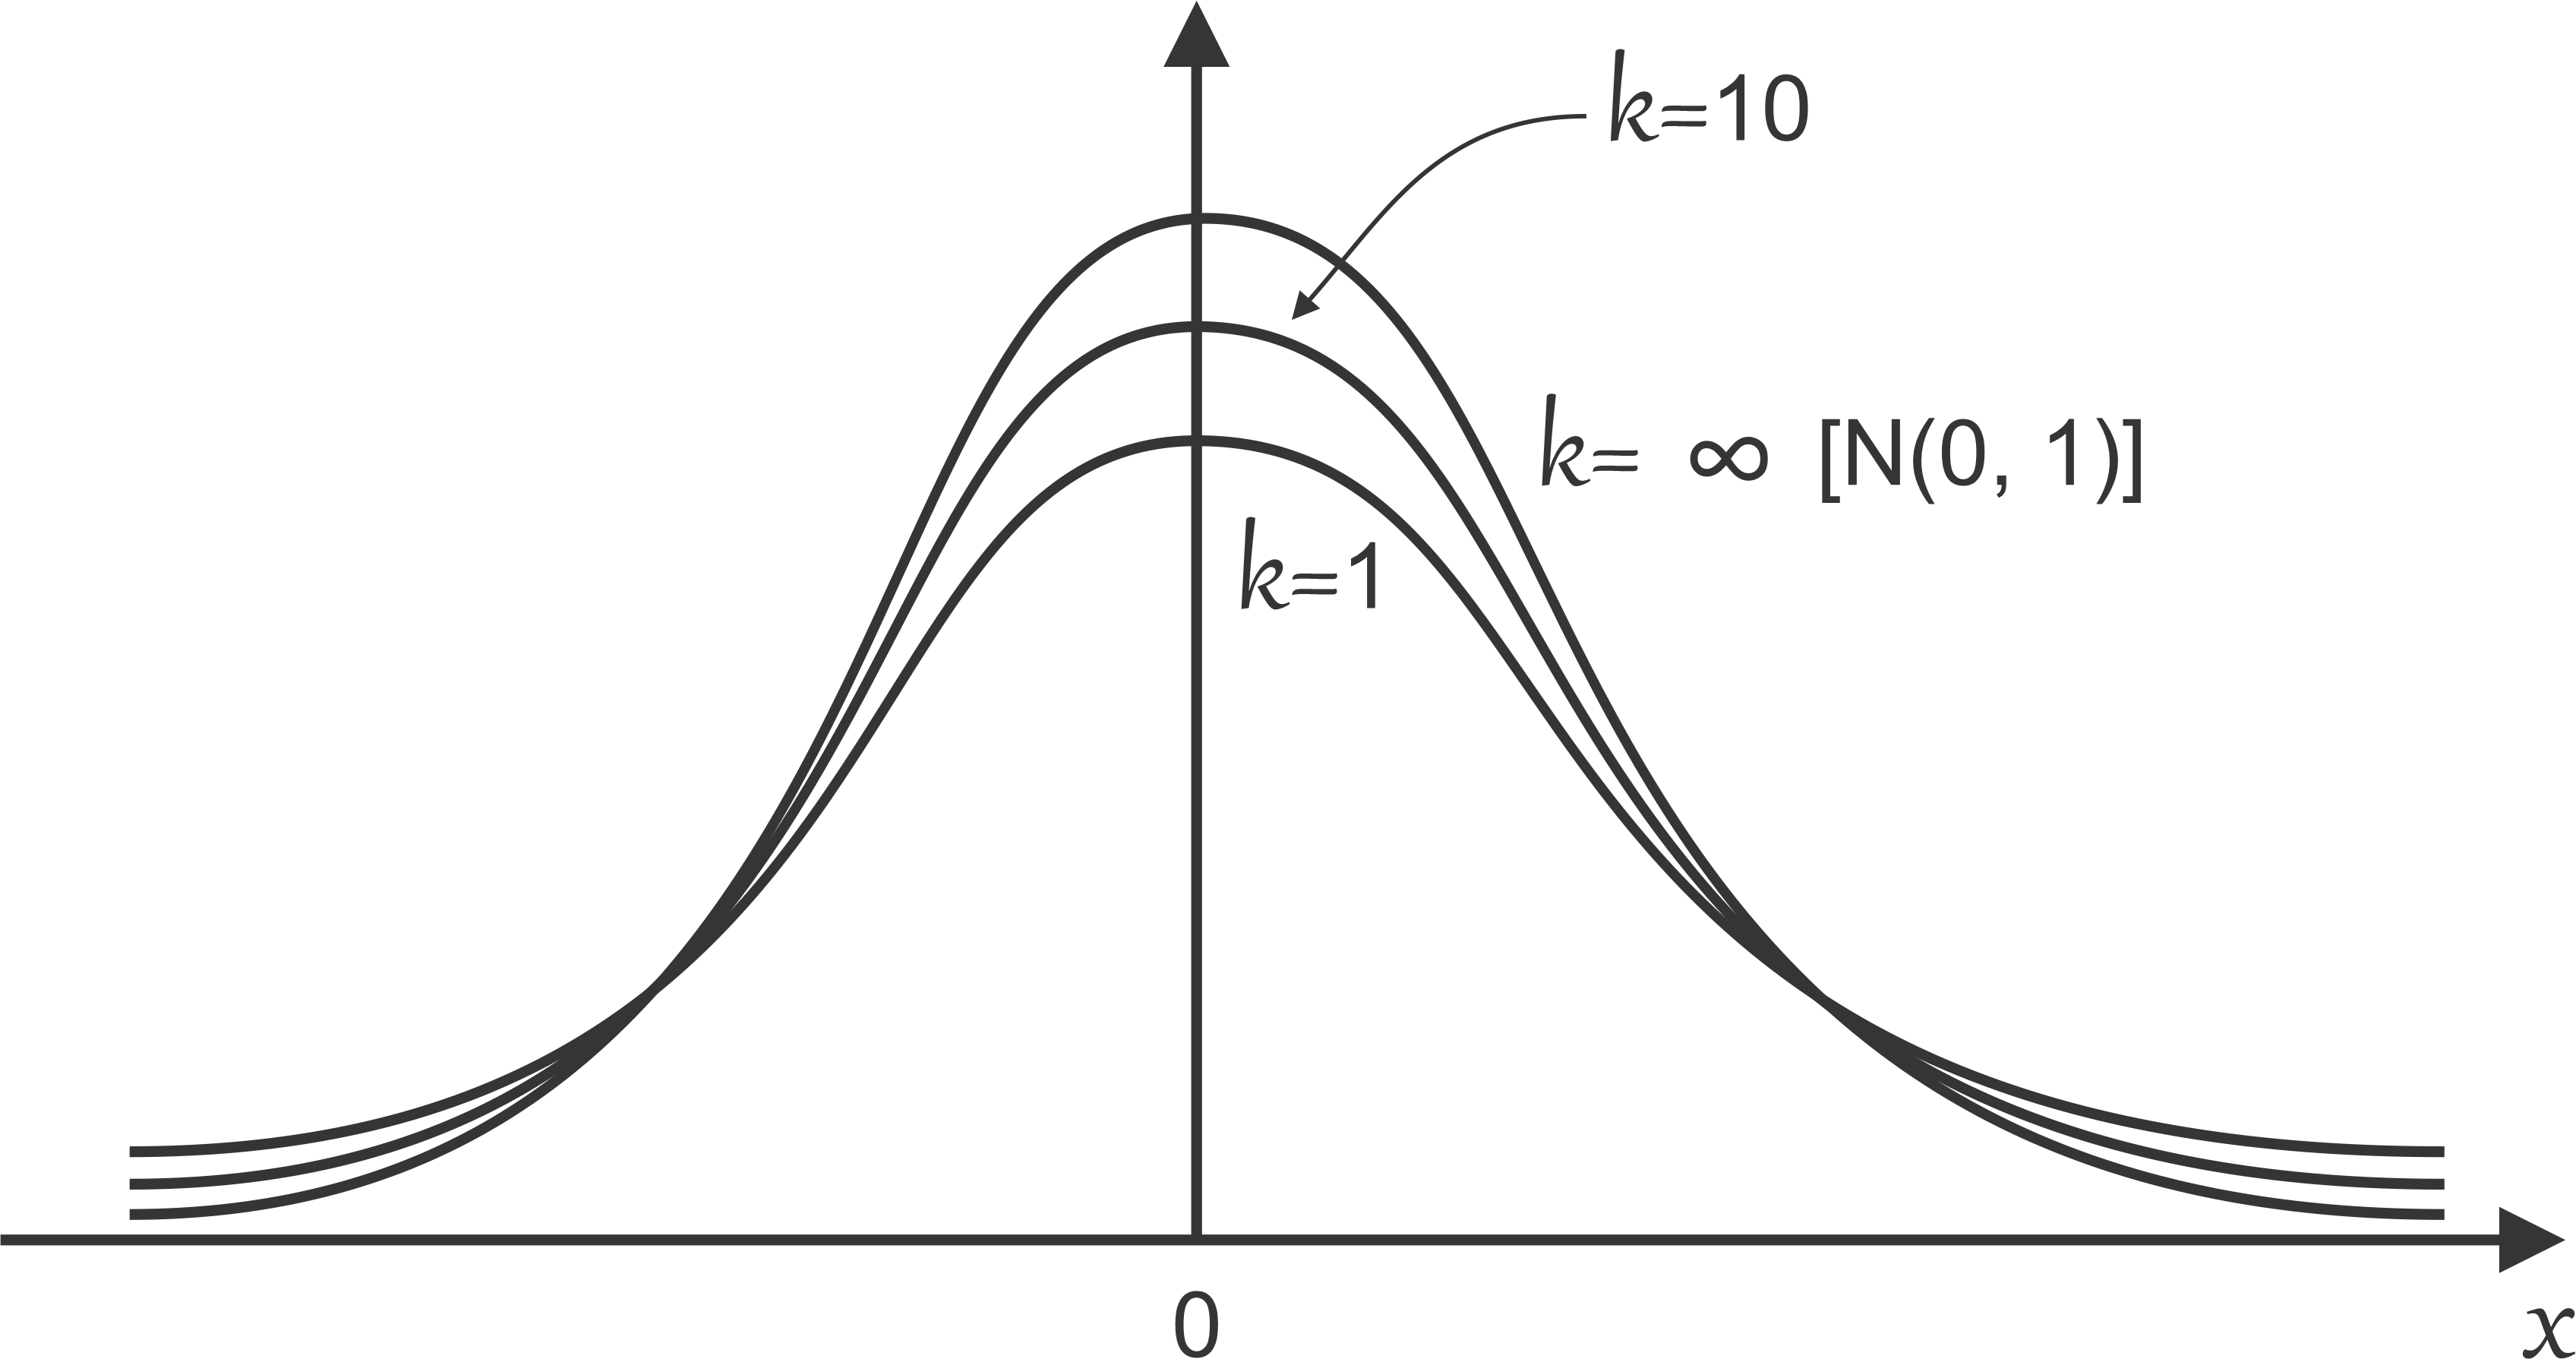
\includegraphics[width=0.7\linewidth]{fig1}
		\caption[]{Funções densidade de probabilidade de várias distribuições t.}
		\label{8.11}
	\end{figure}

	Agora, pode-se ver, de forma direta, que a distribuição da estatística de teste na Eq.8.39 é $t$, com $n-1$ graus de liberdade, se a hipótese nula $H_0: \mu = \mu_0$ for verdadeira. Para testar $H_0: \mu = \mu_0$, o valor da estatística de teste $t_0$ na Eq.8.39 é calculado e $H_0$ é rejeitada se
	\begin{equation}
		\tag{8.41a}
		t_0 > t_{\alpha / 2, n-1}
	\end{equation}
	ou
	\begin{equation}
		\tag{8.41b}
		t_0 < - t_{\alpha / 2, n-1}
	\end{equation}

	em que $t_0 > t_{\alpha / 2, n-1}$ e $t_0 < - t_{\alpha / 2, n-1}$ são pontos $100 \alpha / 2 \%$ superior e inferior da distribuição $t$, com $n-1$ graus de liberdade, definidos previamente.
	
	\hspace*{12pt} Para a hipótese alternativa unilateral
	\begin{equation*}
		H_0: \mu = \mu_0
	\end{equation*}
	
	\begin{equation}
		\tag{8.42}
		H_1: \mu > \mu_0
	\end{equation}
	Calculamos a estatística de teste $t_0$, a partir da Eq. 8.9, e rejeitamos %H_0% se
	\begin{equation}
		\tag{8.43}
		t_0 >  t_{\alpha, n-1}
	\end{equation}

	Para a outra hipótese alternativa unilateral
	\begin{equation*}
		H_0: \mu = \mu_0
	\end{equation*}
	\begin{equation}
		\tag{8.44}
		H_1: \mu < \mu_0
	\end{equation}

	\begin{figure}[H]
		\centering
		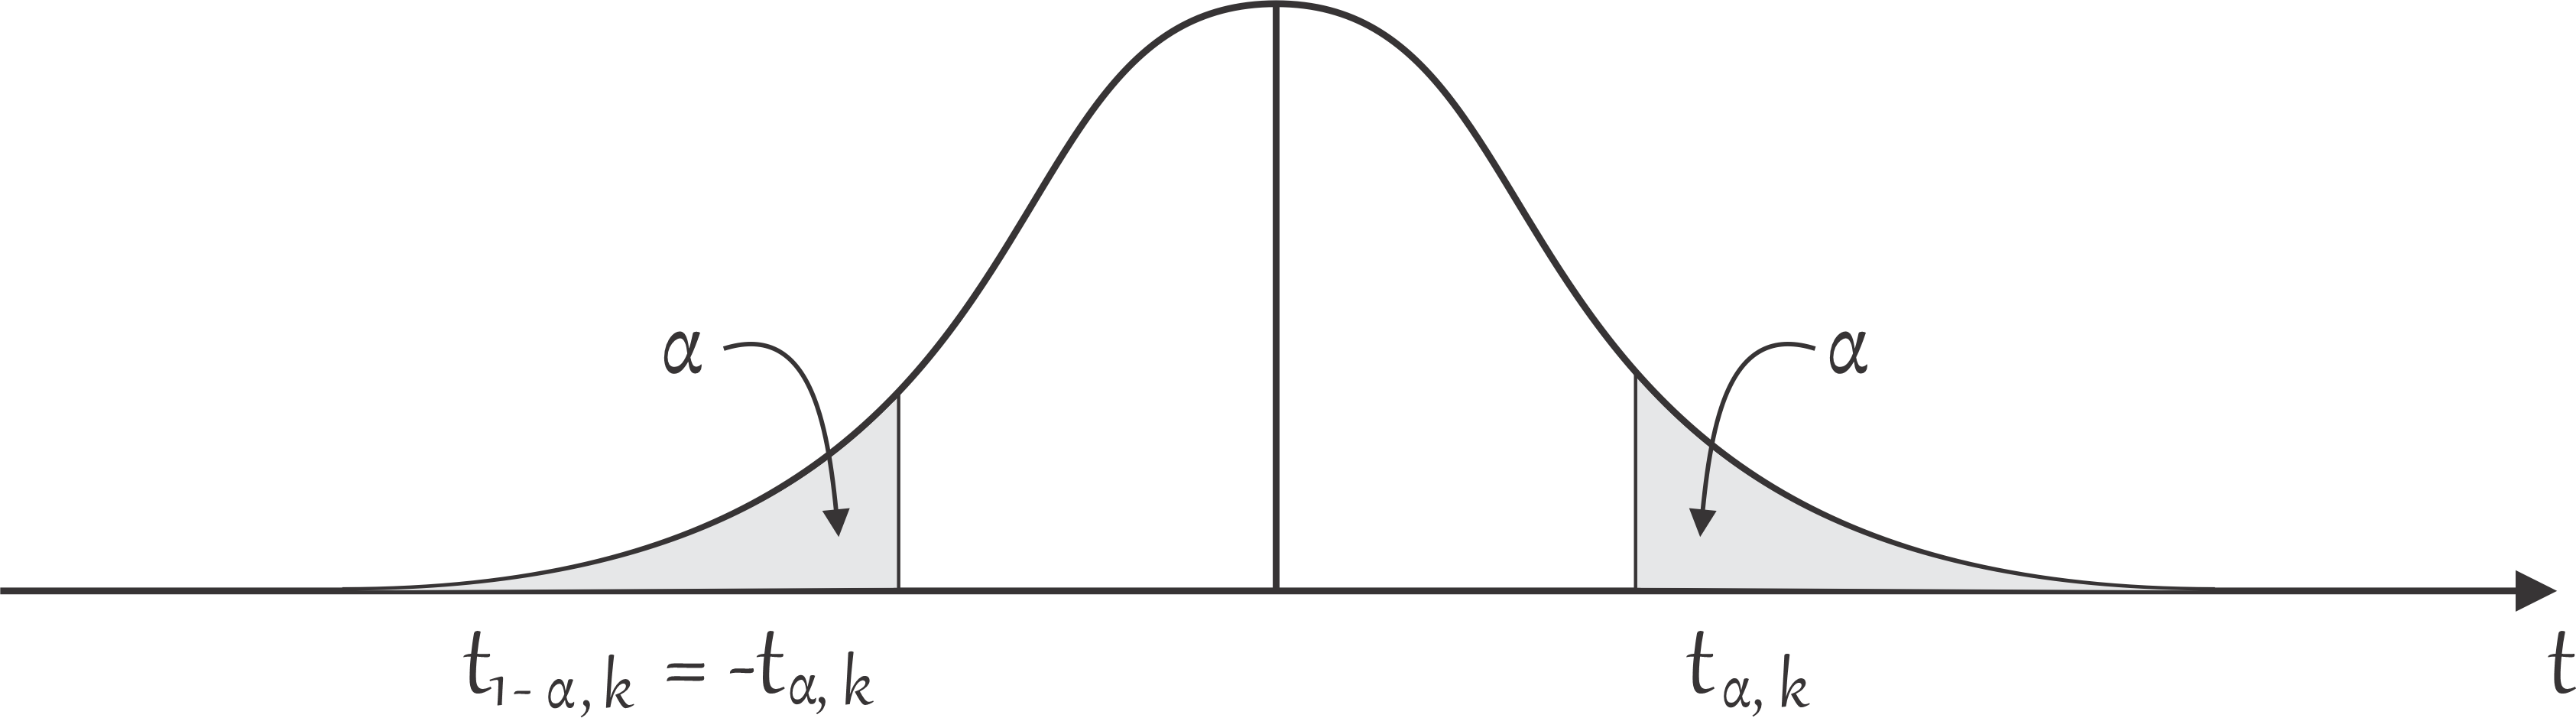
\includegraphics[width=0.7\linewidth]{fig2}
		\caption[]{pontos percentuais da distribuições t.}
	
	\end{figure}

	rejeitamos $H_0$ se
	\begin{equation}
		\tag{8.45}
		t_0 < -t_{\alpha, n-1}
	\end{equation}
	

	
	
	
\end{document}
	